\section{Abstract Syntax Trees}
\label{sec:AST}

Instead of analyzing the code on the higher level or using some internal representation between assembly and high-level code, we have decided to use the \emph{Abstract syntax trees} (\emph{AST} from now on).

\begin{defn}
    An \emph{abstract syntax tree} is a tree representation of the abstract syntactic structure of source code written in a programming language. Each node of the tree denotes a construct occurring in the source code.
\end{defn}

\begin{exmp}
    \textit{Consider the following code snippet:}

    \begin{lstlisting}
    while (x < 20) {
        x = x + y * 2
    }
    \end{lstlisting}

    \textit{The appropriate AST can be seen on figure \ref{fig:WhileAST}.}

\qed
\end{exmp}

\begin{figure}
    \centering
    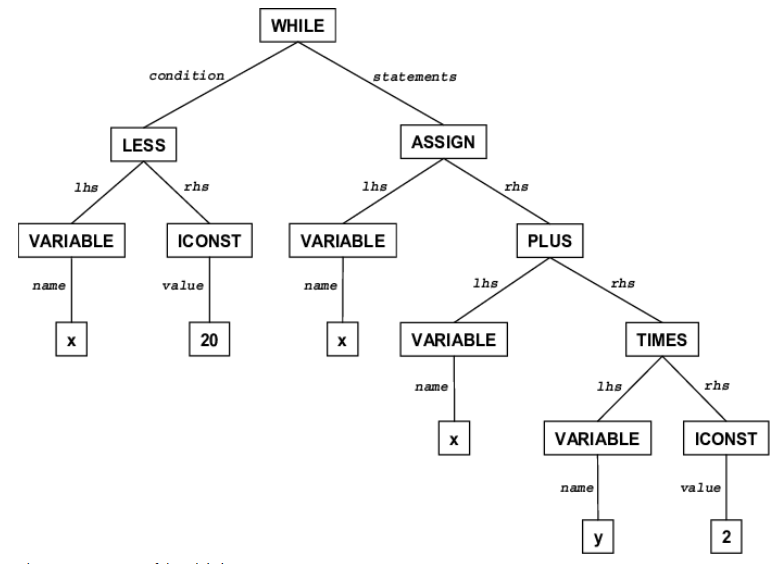
\includegraphics[scale=0.6]{res/WhileAST.PNG}
    \caption{AST for the while loop}
    \label{fig:WhileAST}
\end{figure}

Using the AST instead of the pure code has many advantages. Namely, different code snippets might have the same AST representation which itself does the job of semantical analysis. This is a rare case though, however it is still easier to compare the trees instead of code samples because the tree structure does not contain redundancies like whitespace for example. Also, there exist libraries for AST creation which we use and describe in the following chapter.
